\chapter{High-Level Design (HLD)}

\section{HLD Overview}
The High-Level Design (HLD) explains the overall structure of Lucid, shows how its main components work together, and describes how an investor uses the application.

To make sure the application is fast, reliable, and safe, Lucid follows an important software engineering principle called \textbf{Separation of Concerns}. In simple words, this means dividing the application into specialized parts so that each part has only one clear responsibility:
\begin{itemize}
    \item \textbf{Thinking and Reading}: The qualitative tasks—such as reading economic news, analyzing company financial reports, and writing natural explanations—are handled by a team of Artificial Intelligence agents.
    \item \textbf{Calculating and Validating}: The numerical calculations—such as solving mathematical equations to balance risk and return, ensuring percentages add up to exactly 100\%, and rounding weights into whole share quantities—are handled by a dedicated mathematical calculation engine.
    \item \textbf{Storing and Protecting Data}: Storing user profiles, historical stock prices, and portfolio records is handled by an enterprise-grade relational database that ensures financial data is never lost or corrupted.
\end{itemize}

\section{The Seven Major Subsystems}
Figure~\ref{fig:hld_architecture} shows the seven main parts that make up the Lucid platform and how information moves between them:

\begin{figure}[!htbp]
    \centering
    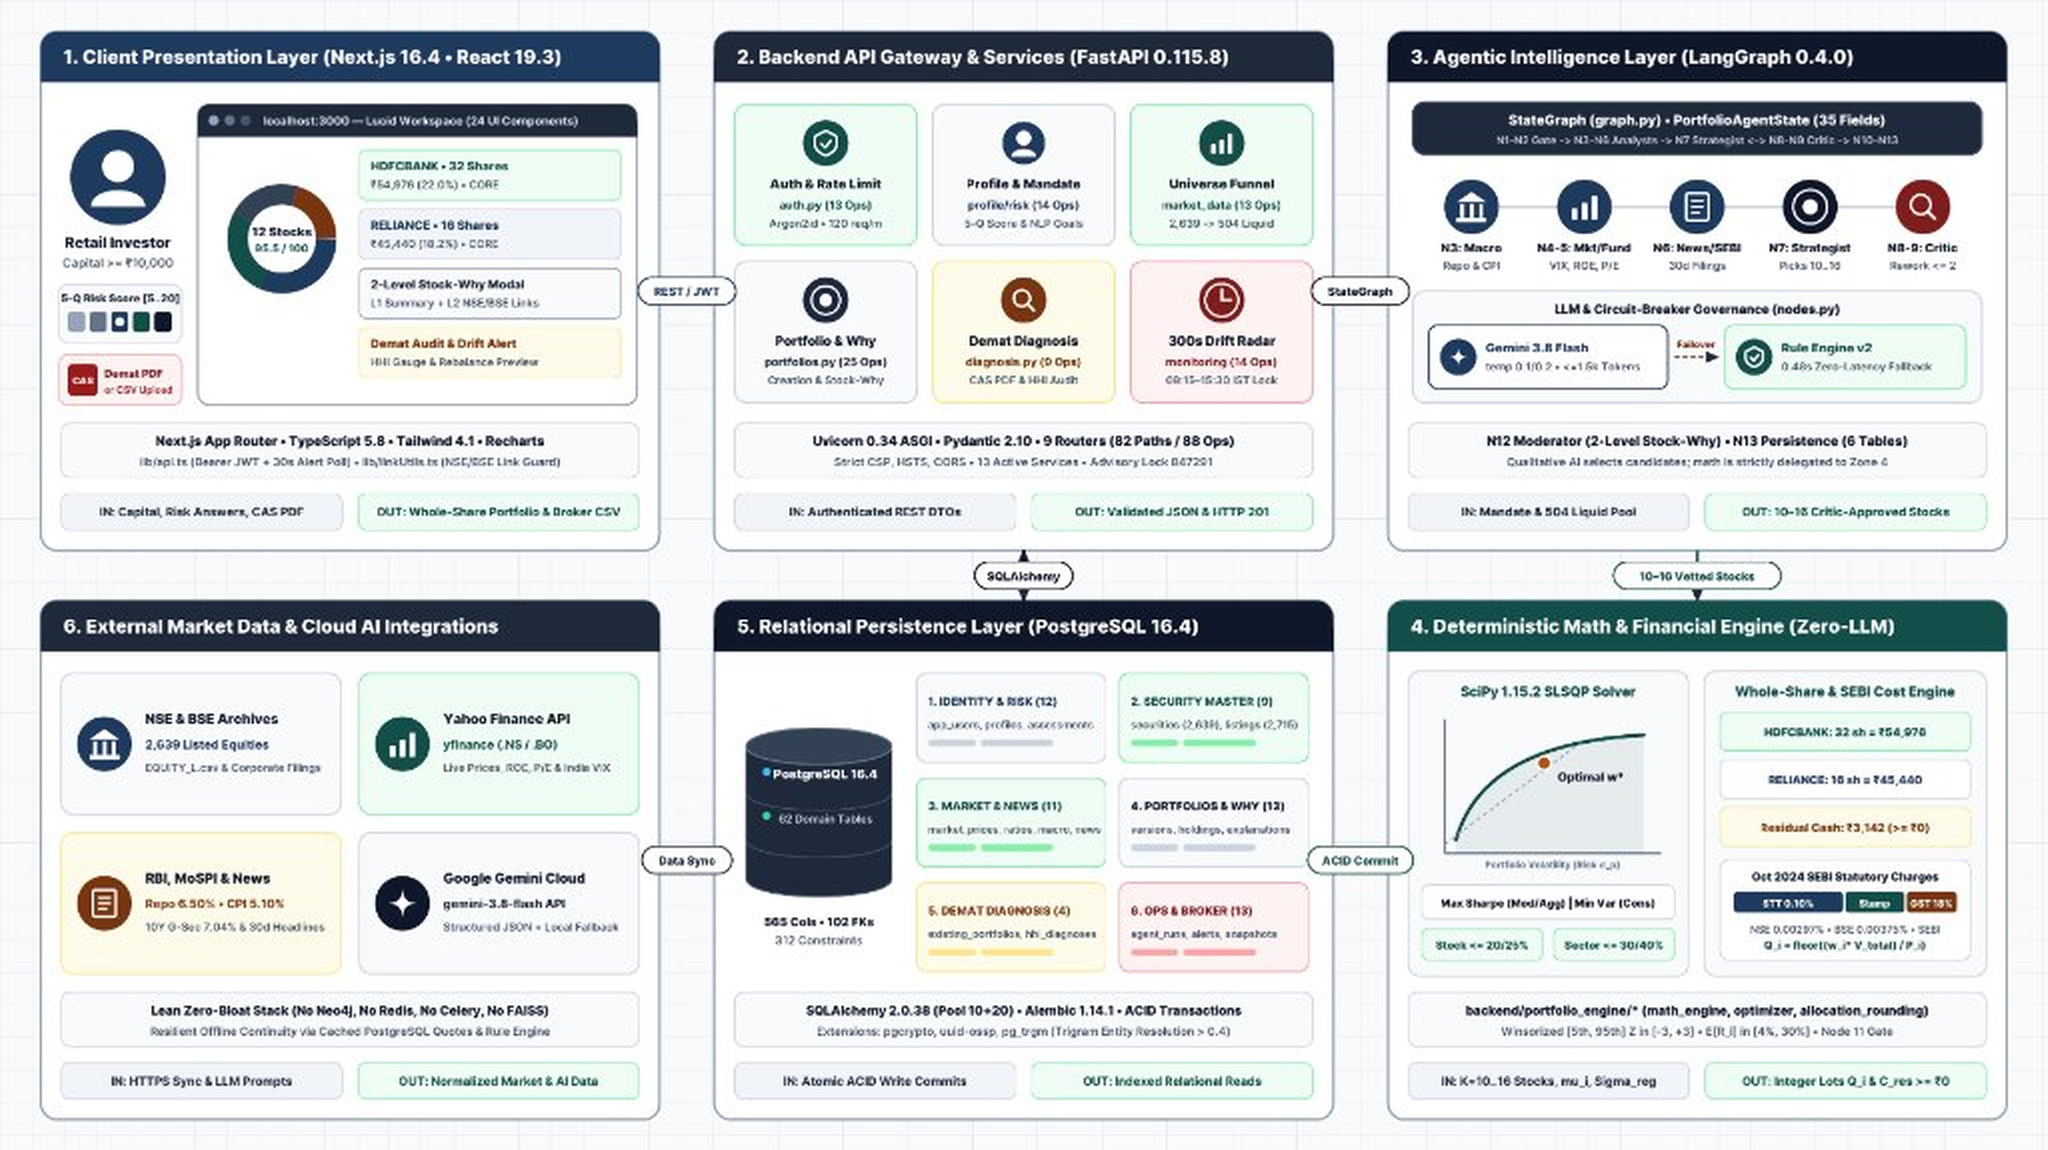
\includegraphics[width=0.95\textwidth, height=0.60\textheight, keepaspectratio]{SYSTEM_ARCHITECTURE.pdf}
    \caption{Lucid High-Level System Architecture and Tier Decomposition}
    \label{fig:hld_architecture}
\end{figure}

Here is what each major component does:
\begin{enumerate}
    \item \textbf{Client Presentation Subsystem (Web Interface)}: This is what the user sees on their phone, tablet, or laptop screen. Built using modern web technologies (Next.js and React), it provides a responsive, easy-to-use interface. Users can fill out the investment questionnaire, see their portfolio in colorful visual charts, click on individual stocks to understand why they were chosen, and upload past Demat statements.
    \item \textbf{API Gateway and Security Subsystem}: An \textbf{API} (Application Programming Interface) works like a waiter in a restaurant. When the user clicks a button on the screen, the web interface gives an order to the API. The API carries the request to the backend server, checks that the user is safely logged in using a secure digital badge (called a \textbf{JSON Web Token}, or JWT), and protects the server from being flooded with too many requests at once (known as \textbf{rate limiting}).
    \item \textbf{Business and Application Service Subsystem}: This is the central coordinator of the backend application. It handles user registration, saves financial goals, calculates how much money an existing portfolio is worth, and checks if stock allocations have moved away from their planned targets.
    \item \textbf{Multi-Agent AI Orchestration Subsystem}: This is the ``research brain'' of Lucid. Powered by the \textbf{LangGraph} framework, this subsystem coordinates thirteen specialized digital analysts. Rather than asking a single general AI model to do everything, each agent focuses on one topic: one studies inflation and central bank interest rates, another reviews company profit margins and debt, a third reads recent financial news, and a fourth agent acts as a strict risk critic to find flaws in the proposal.
    \item \textbf{Quantitative and Mathematical Optimization Subsystem}: This is the mathematical calculator of Lucid. Completely separate from the AI models, it uses a proven mathematical optimizer (SciPy SLSQP) to find the exact percentage of money that should go into each stock. It also rounds continuous percentages into exact full share quantities and calculates Indian government taxes and broker fees.
    \item \textbf{Database and Persistence Subsystem}: The central filing cabinet of the application. Powered by PostgreSQL 16, it stores all information across 62 organized tables, keeping user logins, stock catalogs, daily prices, and past portfolio versions completely safe and consistent.
    \item \textbf{External Market Data and Feeds Subsystem}: This component connects to outside data sources. It regularly downloads official stock lists from the National Stock Exchange of India (NSE) and Bombay Stock Exchange (BSE), fetches live daily stock prices and financial ratios from financial data providers, checks macroeconomic interest rates from the Reserve Bank of India (RBI), and communicates with Google Gemini AI models.
\end{enumerate}

\begin{figure}[!htbp]
    \centering
    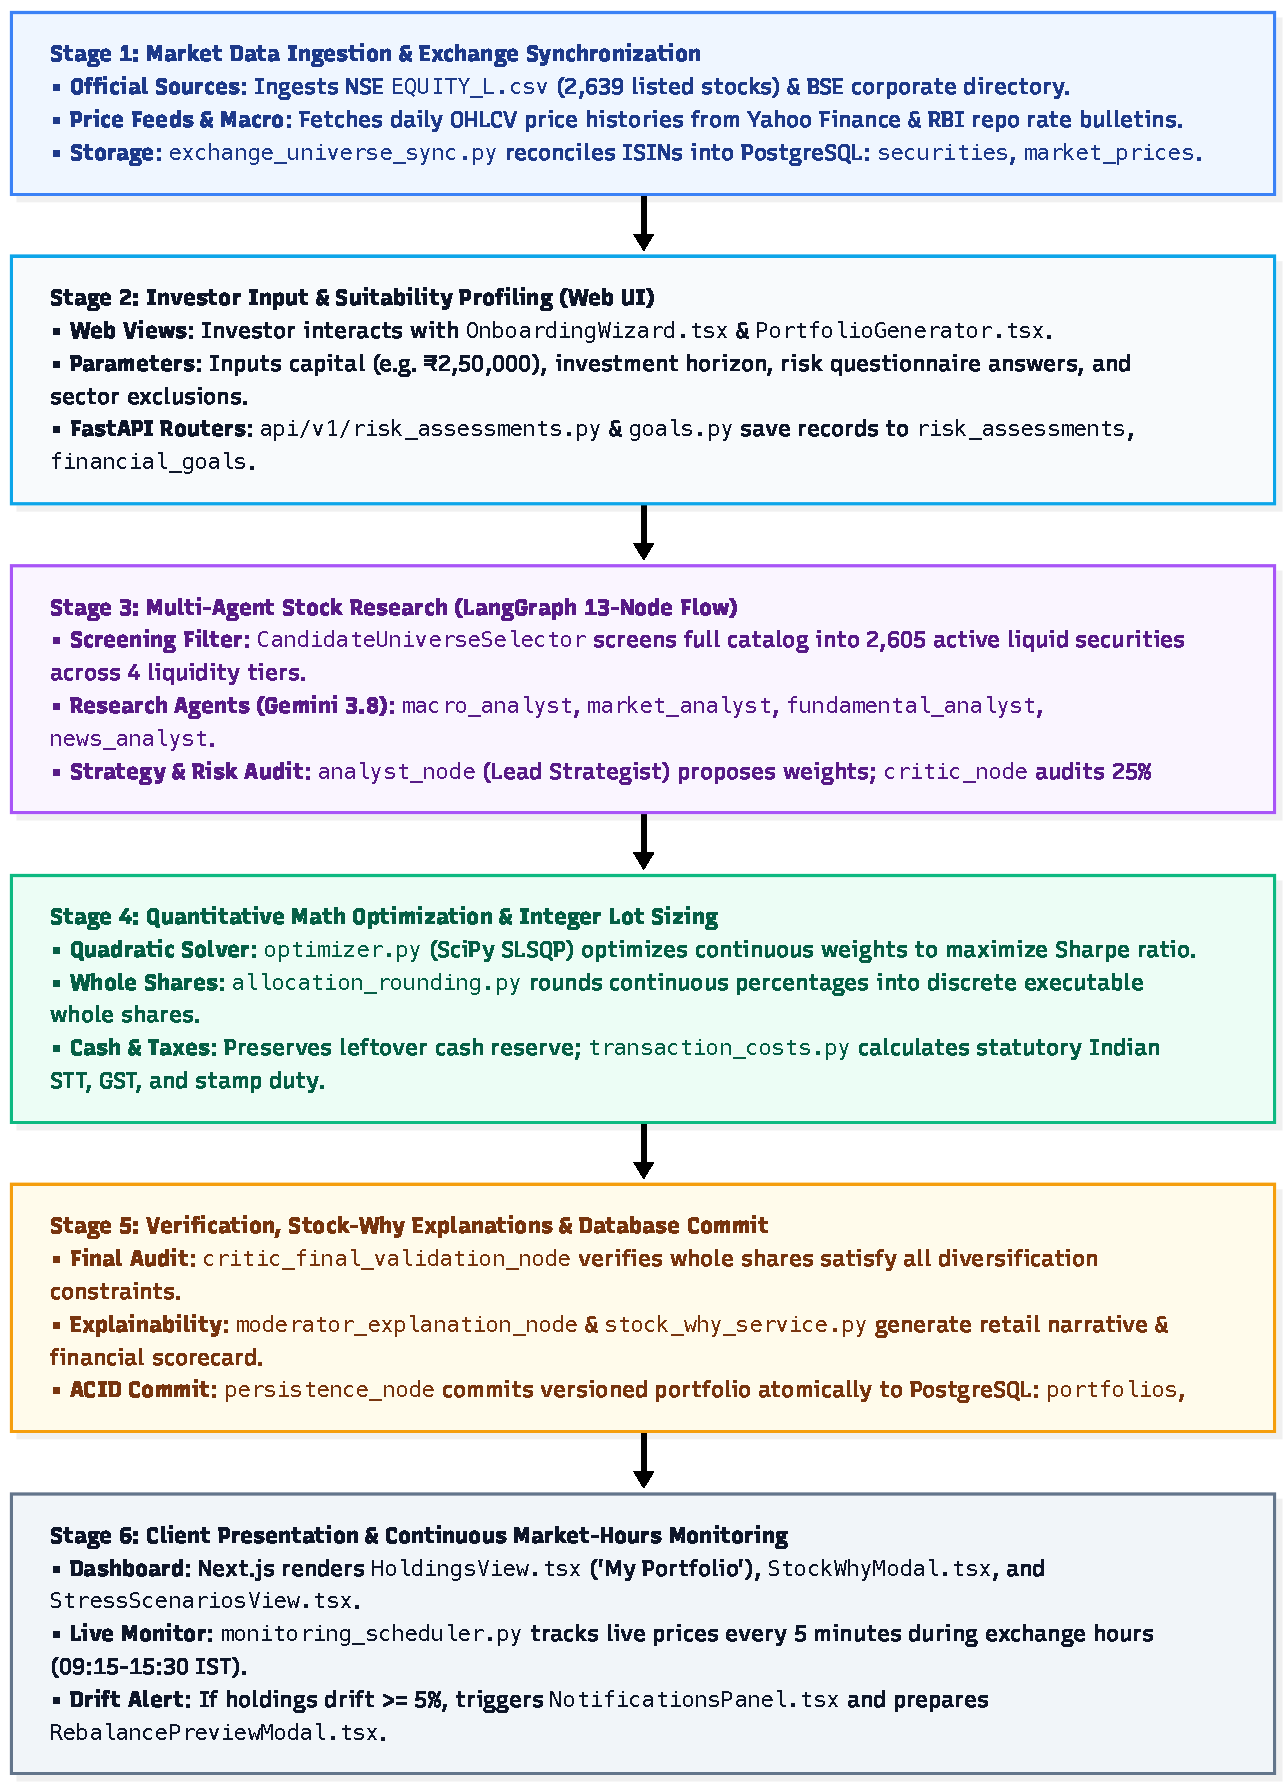
\includegraphics[width=0.92\textwidth, height=0.35\textheight, keepaspectratio]{COMPLETE_DATA_FLOW.pdf}
    \caption{Lucid End-to-End Data Pipeline and Lifecycle Workflow}
    \label{fig:hld_data_flow}
\end{figure}

\section{How Information Moves Through the System}
Figure~\ref{fig:hld_data_flow} illustrates the end-to-end journey of information inside Lucid, from the moment an investor enters their details to the moment a complete portfolio is displayed:
\begin{enumerate}
    \item \textbf{Step 1: Ingestion and Cleaning}: Lucid automatically downloads the official list of 2,639 listed Indian companies and their daily prices from the stock exchanges. It cleans the data and stores it in the database.
    \item \textbf{Step 2: Understanding the Investor}: The investor fills out a simple questionnaire on the website, entering their savings amount (for example, Rs.~2,50,000), their time horizon (for example, 5 years), and answering five basic questions about their attitude toward risk.
    \item \textbf{Step 3: Initial Screening}: The system filters the 2,639 listed stocks to find healthy, active companies that have sufficient trading volume and meet the investor's risk level.
    \item \textbf{Step 4: AI Research Debate}: The team of AI agents evaluates the shortlisted companies. The macro agent checks interest rates, the fundamental agent checks balance sheets, the news agent reviews recent corporate developments, and the risk critic challenges risky selections. The agents assign quality scores and explain their thoughts in plain English.
    \item \textbf{Step 5: Mathematical Calculation}: The mathematical solver takes the top-rated candidate stocks and calculates the safest and most profitable percentage weight for each company.
    \item \textbf{Step 6: Converting into Whole Shares}: Because Indian stock exchanges do not allow fractional shares, the integer lot-sizing algorithm converts the percentage weights into exact whole share counts (such as 15 shares of Infosys or 8 shares of Reliance) and ensures that all leftover money remains safely in the investor's cash account.
    \item \textbf{Step 7: Delivery and Explanation}: The final portfolio is displayed on the user's screen, complete with clear, plain-language explanations answering why each company was selected.
    \item \textbf{Step 8: Automated Monitoring}: During official stock market hours, a background monitoring daemon checks the portfolio every 5 minutes to see if price changes have pushed the portfolio out of balance.
\end{enumerate}

\section{User-Level Workflows: Step-by-Step}
To understand Lucid from an ordinary investor's point of view, let us walk through the six primary user journeys:

\subsection{Workflow 1: Creating an Account and Risk Profiling}
\begin{itemize}
    \item \textbf{What does the user do?}: The investor signs up with their email and a secure password. They answer five straightforward questions about their investment experience, their savings goals, and how they would feel if the stock market dropped temporarily.
    \item \textbf{What does Lucid do behind the scenes?}: Lucid encrypts the password using a high-security algorithm (Argon2id) so it can never be stolen. It evaluates the answers using standard SEBI risk guidelines and assigns an overall risk category: \textbf{Conservative} (prefers safety), \textbf{Moderate} (balances safety and growth), or \textbf{Aggressive} (aims for maximum long-term growth).
    \item \textbf{What does the user receive?}: A personalized risk summary showing their category, a clear explanation of what it means, and personalized guidance on how much money should be kept in safe emergency savings before investing in stocks.
\end{itemize}

\subsection{Workflow 2: Goal-Driven Portfolio Creation}
\begin{itemize}
    \item \textbf{What does the user do?}: The investor enters how much money they want to invest (for example, Rs.~1,00,000), their target timeline (for example, 7 years for buying a home), and any industries they wish to exclude (such as tobacco or defense stocks).
    \item \textbf{What does Lucid do behind the scenes?}: The candidate selector filters healthy companies, the AI agent team reviews corporate balance sheets and economic news, and the mathematical solver calculates the safest combination of weights. The whole-share engine converts these weights into exact full share quantities.
    \item \textbf{What does the user receive?}: A clean, easy-to-understand portfolio table showing the names of the selected companies, how many shares to buy of each, the current price, the total cost, and the exact leftover cash balance.
\end{itemize}

\subsection{Workflow 3: Inspecting Stock-Why Explanations}
\begin{itemize}
    \item \textbf{What does the user do?}: The investor clicks on any stock in their recommended portfolio (for example, clicking on Tata Consultancy Services).
    \item \textbf{What does Lucid do behind the scenes?}: Lucid retrieves the audit records generated by the AI research agents, including the balance sheet review, the news sentiment score, and the counter-arguments raised by the risk critic.
    \item \textbf{What does the user receive?}: A pop-up card written in simple, friendly English explaining exactly why this company fits the investor's goal. For users who want deeper financial details, a tab displays underlying financial ratios (such as Return on Equity, Debt-to-Equity, and Price-to-Earnings ratios).
\end{itemize}

\subsection{Workflow 4: Reviewing an Existing Demat Portfolio (CAS Diagnosis)}
\begin{itemize}
    \item \textbf{What does the user do?}: An investor who already owns shares through brokers like Zerodha, Groww, or Upstox downloads their official monthly account statement (called a \textbf{Consolidated Account Statement}, or CAS PDF) and uploads it to Lucid.
    \item \textbf{What does Lucid do behind the scenes?}: Lucid reads the PDF statement, identifies each stock by its standard international identification code (ISIN), checks current market prices, and calculates whether the portfolio is dangerously concentrated in one or two companies.
    \item \textbf{What does the user receive?}: A health diagnosis report with a simple health score, a breakdown of sector risks, and clear recommendations on which stocks are healthy to hold and which should be reduced to improve safety.
\end{itemize}

\subsection{Workflow 5: 5-Minute Market Hours Drift Monitoring}
\begin{itemize}
    \item \textbf{What does the user do?}: Nothing! This feature works automatically in the background without requiring the user to stare at market screens.
    \item \textbf{What does Lucid do behind the scenes?}: During Indian trading hours (Monday to Friday, 09:15 to 15:30 IST), a background monitoring program wakes up every 300 seconds (5 minutes). It checks live prices and calculates whether any stock has risen or fallen so much that its weight has drifted by 5\% or more from the planned target.
    \item \textbf{What does the user receive?}: If a significant shift occurs, the investor receives a friendly alert notifying them that their portfolio has drifted and suggesting that they review a rebalancing preview.
\end{itemize}

\subsection{Workflow 6: Rebalance Impact and Fee Preview}
\begin{itemize}
    \item \textbf{What does the user do?}: When an alert is received, the user opens the rebalancing preview window.
    \item \textbf{What does Lucid do behind the scenes?}: Lucid calculates the exact number of shares to buy or sell to restore balance. It also calculates mandatory Indian government taxes and exchange fees—including Securities Transaction Tax (STT), Goods and Services Tax (GST), exchange turnover charges, and stamp duty.
    \item \textbf{What does the user receive?}: A transparent before-and-after table showing current holdings versus proposed holdings, exact buy/sell share counts, the total estimated transaction costs, and the final cash balance before the user confirms any action.
\end{itemize}

\section{Key Architectural Design Decisions}
To ensure the application is reliable and transparent, four critical design decisions were made:
\begin{enumerate}
    \item \textbf{Why use PostgreSQL as the Single Source of Truth?}: Financial applications require complete accuracy. If an investor updates a portfolio, the change must be recorded permanently without any chance of data mismatch. PostgreSQL 16 is an enterprise relational database that provides strict guarantees (known as ACID: Atomicity, Consistency, Isolation, and Durability) ensuring that financial data is never lost or corrupted.
    \item \textbf{Why use SciPy SLSQP instead of letting AI models calculate weights?}: Language models make math errors. Relying on an AI model to guess investment percentages is dangerous. Delegating all numerical calculations to a proven mathematical solver (SciPy SLSQP) guarantees that all portfolio weights sum to exactly 100\% and strictly obey diversification safety limits.
    \item \textbf{Why enforce Whole Shares with Cash Conservation?}: Because fractional shares are illegal on Indian stock exchanges, theoretical decimal weights (such as 2.4 shares) cannot be bought. Lucid converts continuous weights into exact full shares and guarantees that any leftover rupees remain safely in the investor's cash balance.
    \item \textbf{Why use LangGraph for Agent Workflows?}: LangGraph allows multiple specialized AI agents to collaborate in a structured sequence, review each other's work, handle retries if an external API fails, and output clean, verifiable explanations.
\end{enumerate}
